\documentclass[runningheads]{llncs}

\usepackage[T1]{fontenc}
\usepackage{graphicx}
\usepackage{amsmath}
\usepackage{amssymb}
\usepackage{amsfonts}
\usepackage{quantikz}

\usepackage{float}
\begin{document}

\title{Qubit Initialization in Variational Quantum Portfolio Optimization: Effects of Circuit Depth and Objective Functions}

\titlerunning{Qubit Initialization in Variational Quantum Portfolio Optimization}

\author{Sumukh J}

\authorrunning{S. J}

\institute{Department of Computer Science, Manipal Institute of Technology Bangalore,
Bangalore, India\\
\email{sumukh.mitblr2024@learner.manipal.edu}}

\maketitle

\begin{abstract}
Selecting asset allocations that jointly optimize return and downside risk remains a central challenge in computational finance, and classical methods scale poorly with the combinatorial complexity of binary asset selection as the number of assets grows. We present a hybrid quantum-classical variational circuit for portfolio optimization, evaluated first on seven and then on twelve NASDAQ-listed assets. Hadamard and computational zero-state qubit initialization are compared under two objective functions --- Expectation value and Conditional Value-at-Risk --- at circuit depths $d \in \{1, 2, 3, 4\}$, across 20 independent random seeds using the Qiskit Aer simulator \cite{qiskit}. Hadamard initialization achieved lower mean portfolio costs at shallow depth, though the effect diminished as depth increased. Circuit depth has a significant effect on solution quality, while initialization does not reach statistical significance at either problem scale. Extended 12-asset experiments ($n = 12$, 320 runs) confirm these results at scale and introduce two convergence metrics --- iterations-to-95\%-optimality ($T_{95}$) and 95\%-success rate ($S_{95}$) --- showing that deeper circuits reach near-optimal solutions in fewer iterations. Statistical significance is assessed via the Wilcoxon signed-rank test.

\keywords{variational quantum algorithms \and portfolio optimization \and qubit initialization \and Hadamard gate \and CVaR \and COBYLA \and Qiskit \and convergence analysis}
\end{abstract}

\section{Introduction}
Selecting a portfolio that achieves an appropriate balance between expected return and financial risk remains one of the central problems in quantitative finance.
\begin{equation}
    \mathcal{C}(\mathbf{w}) = q\mathbf{w}^\top \Sigma \mathbf{w} 
    - (1 - q)\boldsymbol{\mu}^\top \mathbf{w}
\end{equation}
where $\mathbf{w}$ is the portfolio weight vector and $q\in [0,1]$ is the risk parameter. For binary asset selection over $n$ assets, the solution space contains $2^n$ possible portfolios, rendering classical approaches computationally expensive as $n$ grows.

Quantum computing addresses this combinatorial structure by encoding all $2^n$ asset combinations as quantum basis states. A variational quantum circuit represents candidate allocations as superposition states, enabling probabilistic exploration of the solution space. VQAs pair shallow parametrized circuits with classical feedback loops to approximate solutions on noisy hardware \cite{cerezo2021}.

One aspect of VQAs that has received comparatively little attention is the choice of initial quantum state. Two common strategies are the computational zero state $|0\rangle^{\otimes n}$, which fixes all qubits to a definite ground state, and the Hadamard-initialized uniform superposition $|+\rangle^{\otimes n}$, which distributes equal probability across all basis states from the outset \cite{nielsen2010}. Initialization influences convergence in classical optimization, but its role in variational quantum circuits is not well understood.

We investigate the effect of qubit initialization on variational quantum portfolio optimization. Initial experiments use seven NASDAQ-listed assets (AAPL, MSFT, GOOG, AMZN, META, NVDA, TSLA) at circuit depths $d \in \{1, 3\}$, yielding 160 runs; the design is then extended to twelve assets at depths $d \in \{1, 2, 3, 4\}$, yielding 320 additional runs. Hadamard and $|0\rangle$ initialization are compared under two objective functions --- Expectation and Conditional Value-at-Risk (CVaR) \cite{rockafellar2000} --- across 20 independent random seeds. Convergence is quantified by the iterations-to-95\%-optimality metric ($T_{95}$) and the 95\%-success rate ($S_{95}$), using COBYLA with significance assessed via the Wilcoxon signed-rank test.

The remainder of this paper is organized as follows. Section~2 reviews related work.
Section~3 introduces background concepts.
Section~4 describes the methodology.
Section~5 presents the experimental analysis.
Section~6 concludes the paper.

\section{Related Work}

Portfolio optimization has been studied extensively since Markowitz introduced the mean--variance framework \cite{markowitz1952}, which underlies the cost function used here. Because variance penalizes upward and downward deviations equally, downside risk measures such as Value-at-Risk (VaR) and Conditional Value-at-Risk (CVaR) were subsequently proposed \cite{rockafellar2000}. CVaR captures expected losses within the worst-$\alpha$ fraction of outcomes and is used here as an alternative variational objective. We retain the Markowitz quadratic formulation for tractability and incorporate CVaR at the objective-function level of the variational loop.

Two principal variational strategies have emerged for combinatorial optimization. QAOA encodes problem structure directly into a mixer Hamiltonian that alternates with a cost Hamiltonian, enforcing hard constraints through the circuit architecture \cite{Farhi2014}. Hardware-efficient ans\"atze instead use generic parameterized rotation and entanglement layers agnostic to the problem Hamiltonian \cite{kandala2017hardware}; the ansatz used here belongs to this category. Because such circuits lack embedded problem-specific structure, the initial quantum state may play a more visible role in shaping the optimization trajectory, which motivates the comparison studied here.

Barkoutsos et al. \cite{barkoutsos2020} showed that replacing the standard expectation value with CVaR improves solution quality in variational quantum optimization, motivating our use of CVaR as one of two objectives. Their analysis showed CVaR acts as a filter against sampling noise in the finite-shot regime: restricting the objective to the lowest-cost fraction of sampled bitstrings discards high-cost outliers rather than averaging them into the gradient signal. Wang et al. \cite{wang2025} demonstrated that hybrid quantum-classical variational circuits can achieve high-quality portfolio allocations, while Scursulim et al. \cite{scursulim2026} showed VQA performance is sensitive to circuit architecture via a Dicke state ansatz.

A related line of work examines parameter and state initialization in variational circuits. McClean et al. showed that randomly initialized parameterized circuits of sufficient depth exhibit barren plateaus --- regions where the cost gradient vanishes exponentially with system size, making optimization impractical \cite{mcclean2018barren}. Subsequent work has explored structured initialization to mitigate this, including fixed-angle heuristics for QAOA \cite{Wurtz_2021_fixed_angle} and layer-wise training protocols. These studies, however, primarily address initial parameter values $\boldsymbol{\theta}_0$ rather than the initial quantum state $|\psi_0\rangle$ preceding the parameterized layers. The distinction matters: parameter initialization determines where in the landscape the search begins, while state initialization determines the baseline distribution the parameterized layers modify. To our knowledge, no prior work has compared $|0\rangle$ and Hadamard state initialization in variational quantum portfolio optimization across varying circuit depths and objective functions.
\section{Background Concepts}

\subsection{Quantum state representation}
A qubit is represented as
\begin{equation}
    |\psi\rangle = \alpha|0\rangle + \beta|1\rangle, 
\end{equation}
where $\alpha,\beta \in \mathbb{C}$ satisfy $|\alpha|^2+|\beta|^2=1$. Each computational basis state $|z\rangle$ encodes a binary asset allocation vector,
\begin{equation}
    z_i \in \{0, 1\}, \quad z_i = 1 \Rightarrow 
    \text{asset } i \text{ is selected},
\end{equation}
so that the quantum state spans the full binary portfolio configuration space.

\subsection{Hadamard initialization}
The Hadamard gate is defined as
\begin{equation}
    H = \frac{1}{\sqrt{2}} \begin{pmatrix} 1 & 1 \\ 1 & -1 
    \end{pmatrix},
\end{equation}
Applied to all qubits, it produces a uniform superposition over the $2^n$ basis states:
\begin{equation}
    |\psi_0\rangle = \frac{1}{\sqrt{2^n}} 
    \sum_{z \in \{0,1\}^n} |z\rangle.
\end{equation}
Every portfolio configuration then has equal measurement probability.

\subsection{Parameterized $R_Y(\theta)$ Rotations}
The single-qubit $Y$-rotation is
\begin{equation}
    R_Y(\theta) = \begin{pmatrix} 
        \cos(\theta/2) & -\sin(\theta/2) \\ 
        \sin(\theta/2) &  \cos(\theta/2) 
    \end{pmatrix},
\end{equation}
giving, for $|0\rangle$ input,
\begin{equation}
    R_Y(\theta)|0\rangle = \cos(\theta/2)|0\rangle 
    + \sin(\theta/2)|1\rangle,
\end{equation}
with measurement probability
\begin{equation}
    P(1) = \sin^2(\theta/2).
\end{equation}
Each qubit has a trainable parameter $\theta\in[0,2\pi]$, and the full parameter vector is optimized using COBYLA.

We use $R_Y$ rotations instead of $R_X$ or general $U_3$ gates to restrict the circuit to the real-amplitude subspace. Both initialization strategies and CNOT entanglement preserve real amplitudes, so the quantum state remains within $\mathbb{R}^{2^n}$ throughout optimization.

\subsection{Entanglement via CNOT gate}
The CNOT gate,
\begin{equation}
    \text{CNOT} = \begin{pmatrix} 
        1 & 0 & 0 & 0 \\ 
        0 & 1 & 0 & 0 \\ 
        0 & 0 & 0 & 1 \\ 
        0 & 0 & 1 & 0 
    \end{pmatrix},
\end{equation}
is applied sequentially between adjacent qubit pairs to capture pairwise correlations.

Linear nearest-neighbor connectivity is used for hardware compatibility and lower gate overhead: the topology requires only $n-1$ CNOT gates per layer, producing shallower circuits less susceptible to noise accumulation.
\section{Methodology}

\subsection{Problem Formulation}
The portfolio optimization problem is formulated as a combinatorial asset selection task over $n = 7$ NASDAQ-listed equities: AAPL, MSFT, GOOG, AMZN, META, NVDA, and TSLA. Two years of trailing adjusted daily closing prices (retrieved via the Yahoo Finance API \cite{yfinance} using a rolling two-year window ending at the date of data collection, July 2026) are used. The annualized mean return vector $\boldsymbol{\mu} \in \mathbb{R}^n$ and covariance matrix $\Sigma \in \mathbb{R}^{n \times n}$ are computed by scaling daily sample statistics by 252 trading days. For a binary selection vector $\mathbf{z} \in \{0,1\}^n$, assets are equally weighted:

\begin{equation}
w_i = \frac{z_i}{\sum_{j=1}^{n} z_j}, \quad 
\text{whenever } \sum_j z_j > 0
\end{equation}

The portfolio cost function balances risk against return:

\begin{equation}
    \mathcal{C}(\mathbf{w}) = q\,\mathbf{w}^\top 
    \Sigma\,\mathbf{w} - (1-q)\,\boldsymbol{\mu}^\top 
    \mathbf{w}, \quad q = 0.5
\end{equation}

Given the small asset universe, the globally optimal allocation is also obtained
by exhaustive evaluation of all $2^n - 1 = 127$ non-empty portfolios, which provides a classical reference benchmark.
Equal weighting follows directly from the binary encoding, since each measured
bit simply determines whether an asset is included or excluded. Encodings that
allow fractional allocations would require additional qubits and are not considered here.
The risk-return parameter is fixed at $q=0.5$, giving equal importance to
variance minimization and return maximization. A sensitivity analysis with respect to $q$ is left for future work.
The initial 7-asset universe permits exact evaluation of all 127 non-empty
portfolios, enabling computation of the global optimum $\mathcal{C}^*$ and exact approximation ratios. Experiments are then extended to $n=12$, where exhaustive evaluation over 4095 portfolios remains tractable.

\subsection{Variational Quantum Circuit}

The ansatz is constructed over $n = 7$ qubits, one per asset, with an optional initialization stage followed by $d$ variational layers. Each layer applies a trainable $R_Y(\theta_{l,i})$ rotation to every qubit, followed by a nearest-neighbor CNOT ladder coupling qubit $i$ to qubit $i+1$ for $i = 0,\ldots,n-2$. The total parameter count is $d \times n$. All qubits are measured after the final layer, and each bitstring $z \in \{0,1\}^n$ maps to an equally weighted portfolio. The circuit is executed for 1024 shots per evaluation.

\begin{figure}[t]
\centering
\resizebox{\textwidth}{!}{
\begin{quantikz}
\lstick{$|0\rangle$} & \gate{H} & \gate{R_Y(\theta_{1,1})} & \ctrl{1} & \qw      & \gate{R_Y(\theta_{2,1})} & \ctrl{1} & \qw      & \meter{} \\
\lstick{$|0\rangle$} & \gate{H} & \gate{R_Y(\theta_{1,2})} & \targ{}  & \ctrl{1} & \gate{R_Y(\theta_{2,2})} & \targ{}  & \ctrl{1} & \meter{} \\
\lstick{$|0\rangle$} & \gate{H} & \gate{R_Y(\theta_{1,3})} & \qw      & \targ{}  & \gate{R_Y(\theta_{2,3})} & \qw      & \targ{}  & \meter{} \\
\lstick{$|0\rangle$} & \gate{H} & \gate{R_Y(\theta_{1,4})} & \qw      & \ctrl{1} & \gate{R_Y(\theta_{2,4})} & \qw      & \ctrl{1} & \meter{} \\
\lstick{$|0\rangle$} & \gate{H} & \gate{R_Y(\theta_{1,5})} & \qw      & \targ{}  & \gate{R_Y(\theta_{2,5})} & \qw      & \targ{}  & \meter{} \\
\end{quantikz}
}
\caption{Variational ansatz circuit with Hadamard initialization (d=2 shown for clarity). Only the first five qubits are displayed; the pattern extends identically to all seven asset qubits used in the experiments. Each qubit 
corresponds to one asset. For $|0\rangle$ initialization, 
the Hadamard gates are omitted. Each variational layer 
consists of $R_Y$ rotations followed by a linear CNOT 
chain, measured in the computational basis 
after the final layer.}
\label{fig:circuit}
\end{figure}

Fig.~\ref{fig:circuit} illustrates the ansatz for \(d=2\). Hadamard gates are omitted under \(|0\rangle\) initialization.

\subsection{Initialization Strategies}

Two initialization strategies are considered.

\textbf{Zero-state} ($|0\rangle$): All qubits are initialized in $|0\rangle^{\otimes n}$.

\textbf{Hadamard} ($H$): A Hadamard gate \cite{nielsen2010} is applied to every qubit before the first variational layer:

\begin{equation}
    |\psi_0\rangle = H^{\otimes n}|0\rangle^{\otimes n} 
    = \frac{1}{\sqrt{2^n}} \sum_{z \in \{0,1\}^n} |z\rangle
\end{equation}

This places all $2^n$ portfolio configurations at equal amplitude, removing initialization bias before optimization begins.

\subsection{Objective Functions}

\textbf{Expectation value: } Probability-weighted average cost over all sampled bitstrings:

\begin{equation}
    \mathcal{L}_{\text{Exp}}(\boldsymbol{\theta}) = 
    \sum_{z} p_z \cdot \mathcal{C}(\mathbf{w}_z)
\end{equation}

\textbf{CVaR} \cite{barkoutsos2020}\textbf{:} Samples are sorted by ascending cost (most negative first) and the lowest-cost $\alpha = 0.3$ fraction of probability mass is accumulated:

\begin{equation}
    \mathcal{L}_{\text{CVaR}}(\boldsymbol{\theta}) = 
    \frac{\displaystyle\sum_{z \in \mathcal{T}_\alpha} 
    \tilde{p}_z \cdot \mathcal{C}(\mathbf{w}_z)}{P_\alpha}
\end{equation}

where $\tilde{p}_z = \min(p_z, \alpha - P_{\text{prev}})$ allows partial inclusion at the tail boundary, and $P_\alpha$ is the total accumulated tail probability.

We fix $\alpha=0.3$ following Barkoutsos et al. \cite{barkoutsos2020}.

The partial inclusion term \(\tilde{p}_z\) ensures that the cumulative tail probability equals \(\alpha\) exactly under finite-shot sampling.

\subsection{Optimization and Experimental Design}

Parameters are optimized with COBYLA \cite{powell1994}, a derivative-free optimizer suited to noisy objective evaluations. The maximum iteration count is 200, with an initial trust-region radius of \(\rho_0=0.5\).

Each circuit evaluation uses 1024 measurement shots on the Qiskit Aer shot-based simulator (\texttt{AerSimulator}), which samples from the ideal output distribution without hardware noise.

Initial parameters are sampled uniformly from $[0,2\pi]$. Twenty independent seeds are used to account for variability in the optimization trajectories.
The baseline study considers two initialization strategies, two depths $(d\in\{1,3\})$, and two objectives across 20 seeds, yielding 160 runs. The extended study considers $n=12$, four depths $(d\in\{1,2,3,4\})$, and the same initialization and objective combinations, producing 320 additional runs.
Statistical significance is assessed with the Wilcoxon signed-rank test at a nominal significance level of $p<0.05$. All reported $p$-values are uncorrected for multiple comparisons; with 12 tests in the 7-asset study, borderline significant results (e.g., $p \approx 0.04$) should be read as exploratory rather than conclusive.
Convergence is quantified with two metrics. The \textit{iterations-to-95\%-optimality} $T_{95}$ is the first iteration $k$ at which the cumulative best approximation ratio reaches 95\% of the classical optimum:
\begin{equation}
    T_{95} = \min \left\{ k : r_k \geq 0.95 \right\}, \quad
    r_k = \frac{\mathcal{C}_{\text{best}}(k)}{\mathcal{C}^*}
\end{equation}
where $\mathcal{C}_{\text{best}}(k) = \min_{j \leq k} \mathcal{C}_j$ is the cumulative minimum cost at iteration $k$; if $r_k$ never reaches $0.95$, $T_{95}$ is set to the maximum iteration count (200). When $S_{95}$ is low (e.g., $\leq 0.10$), most seeds hit this ceiling value, so $T_{95}$ reflects the iteration cap rather than a genuine convergence time; it is most informative when $S_{95} \geq 0.50$. The \textit{95\%-success rate} $S_{95}$ is the fraction of seeds that achieve $r \geq 0.95$ at termination:
\begin{equation}
    S_{95} = \frac{1}{N_{\text{seeds}}} \sum_{s=1}^{N_{\text{seeds}}} \mathbf{1}[r_s \geq 0.95]
\end{equation}
\section{Results and Analysis}

All 160 optimization runs completed successfully across the eight configurations. The globally optimal portfolio cost, obtained by exhaustive evaluation of all $2^n -1 = 127$ non-empty binary portfolios, was $\mathcal{C}^* = -0.17435$, which serves as the classical reference benchmark. All eight configurations reached this optimum in at least one seed; what distinguishes them is average-case performance and consistency.

\subsection{Summary of Results}

Table~\ref{tab:summary} reports, per configuration, aggregate statistics across 20 seeds, including the approximation ratio $r = \overline{\mathcal{C}}_{\text{best}} /\mathcal{C}^*$, where a value of $1.0$ indicates perfect average recovery of the global optimum.
\begin{table}[t]
\caption{Per configuration summary statistics across 20 seeds. $r$ denotes the approximation ratio relative to the classical optimum $\mathcal{C}^* = -0.17435$.}
\label{tab:summary}
\centering
\resizebox{\textwidth}{!}{%
\begin{tabular}{lllllllll}
\hline\textbf{Init} & \textbf{$d$} & \textbf{Obj} &
\textbf{Mean Cost} & \textbf{Std} &
\textbf{$r$} &
\textbf{Mean Obj} & \textbf{Time (s)} &
\textbf{NFEv} \\
\hline
$H$         & 1 & Exp  & $-0.1508$ & $0.0151$ & $0.865$ & $-0.1223$ & $0.120$ & $77.9$ \\
$H$         & 1 & CVaR & $-0.1431$ & $0.0159$ & $0.821$ & $-0.0887$ & $0.111$ & $72.8$ \\
$H$         & 3 & Exp  & $-0.1689$ & $0.0096$ & $0.969$ & $-0.1421$ & $0.424$ & $194.1$ \\
$H$         & 3 & CVaR & $-0.1645$ & $0.0131$ & $0.944$ & $-0.0953$ & $0.411$ & $190.6$ \\
$|0\rangle$ & 1 & Exp  & $-0.1453$ & $0.0190$ & $0.833$ & $-0.1319$ & $0.109$ & $79.5$ \\
$|0\rangle$ & 1 & CVaR & $-0.1421$ & $0.0203$ & $0.815$ & $-0.0917$ & $0.100$ & $71.2$ \\
$|0\rangle$ & 3 & Exp  & $-0.1695$ & $0.0089$ & $0.972$ & $-0.1433$ & $0.407$ & $197.5$ \\
$|0\rangle$ & 3 & CVaR & $-0.1582$ & $0.0117$ & $0.907$ & $-0.0899$ & $0.402$ & $189.7$ \\
\hline
\end{tabular}%
}
\end{table}
Two patterns emerge from Table~\ref{tab:summary}. First, CVaR mean objective values ($-0.088$ to $-0.095$) are less negative than Expectation values ($-0.122$ to $-0.143$), since CVaR optimizes only the worst-$\alpha$ tail rather than the full distribution. Even so, CVaR yields competitive best-cost and approximation-ratio values despite optimizing only the tail of the sampled distribution. Second, increasing depth reduces both the mean and variance of best cost, regardless of initialization or objective.
Figure~\ref{fig:boxplot} shows the distribution of best costs across the $20$ independent seeds for all configurations. At $d=3$, the variance and interquartile range are much smaller than at $d=1$. Median performance approaches the theoretical optimum under both initialization strategies when $d=3$, whereas $d=1$ runs show numerous high-cost outliers --- shallow circuits are more prone to local minima, and the deeper circuit visibly mitigates this problem.
\begin{figure}[h!]
\centering
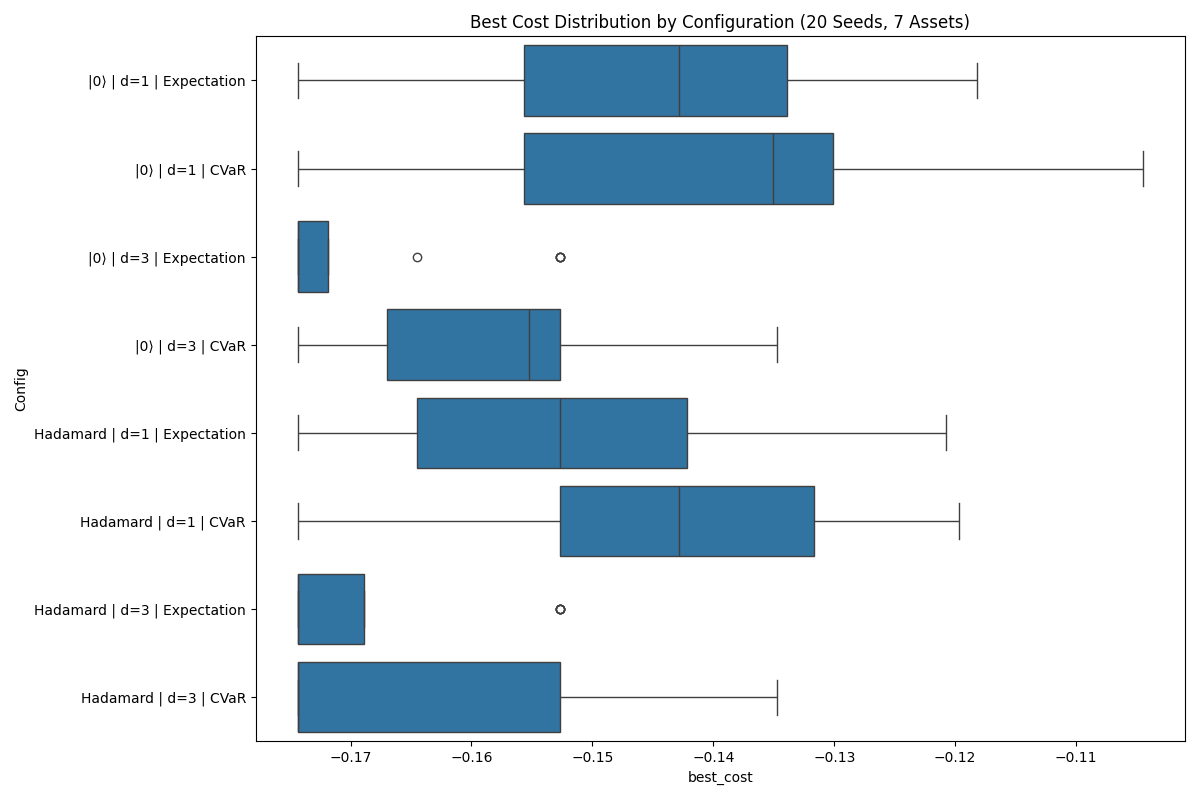
\includegraphics[width=\textwidth]{boxplot.png}
\caption{Distribution of best portfolio costs achieved across 20 independent seeds. Configurations are grouped by objective function, circuit depth, and initialization strategy. The red dashed line denotes the globally optimal portfolio cost $\mathcal{C}^* = -0.17435$.}
\label{fig:boxplot}
\end{figure}

\subsection{Effect of Initialization Strategy}

At circuit depth $d = 1$, Hadamard initialization achieves a slightly better mean best cost than $|0\rangle$ under both objectives: $-0.1508$ versus $-0.1453$ for Expectation, and $-0.1431$ versus $-0.1421$ for CVaR. It also exhibits lower variability ($0.0151$ vs.\ $0.0190$ for Expectation; $0.0159$ vs.\ $0.0203$ for CVaR), indicating more consistent convergence at shallow depth.
With only $d \times n = 7$ parameters, the circuit has limited ability to reshape the probability distribution independently of its initial state. These differences, however, are not statistically significant (Section~\ref{sec:stats}).

At depth $d = 3$, the differences between initialization strategies diminish. Under Expectation, $|0\rangle$ slightly overtakes Hadamard ($-0.1695$ vs.\ $-0.1689$; $r = 0.972$ vs.\ $0.969$), while under CVaR, Hadamard retains an advantage over $|0\rangle$ ($-0.1645$ vs.\ $-0.1582$; $r = 0.944$ vs.\ $0.907$). With 21 parameters at depth 3, the ansatz appears to have enough capacity to reduce its dependence on the initial state.

\subsection{Effect of Circuit Depth}

Increasing depth from $d = 1$ to $d = 3$ improves mean best cost across all four combinations, at the cost of $3.5$--$4.0\times$ longer runtime and $2.4$--$2.7\times$ more function evaluations. The largest gain occurs for $|0\rangle$-Expectation: mean best cost improves from $-0.1453$ to $-0.1695$ ($r$ from $83.3\%$ to $97.2\%$). For Hadamard-CVaR, the gain is from $-0.1431$ to $-0.1645$ ($r$ from $82.1\%$ to $94.4\%$). A single layer provides only 7 rotation parameters and one entanglement round; tripling the depth to 21 parameters and three entanglement rounds substantially expands the expressible hypothesis space.

Figure~\ref{fig:convergence} plots the average convergence across all $20$ seeds, showing the cumulative minimum objective value against COBYLA function evaluations. The $d=3$ configurations reach lower cost values than $d=1$. Shallow circuits often plateau early because of their limited expressibility, whereas $d=3$ runs sustain a steeper descent before levelling off closer to the theoretical minimum. Final values depend mainly on depth, while the convergence trajectories themselves look similar across initialization strategies.

\begin{figure}[h!]
\centering
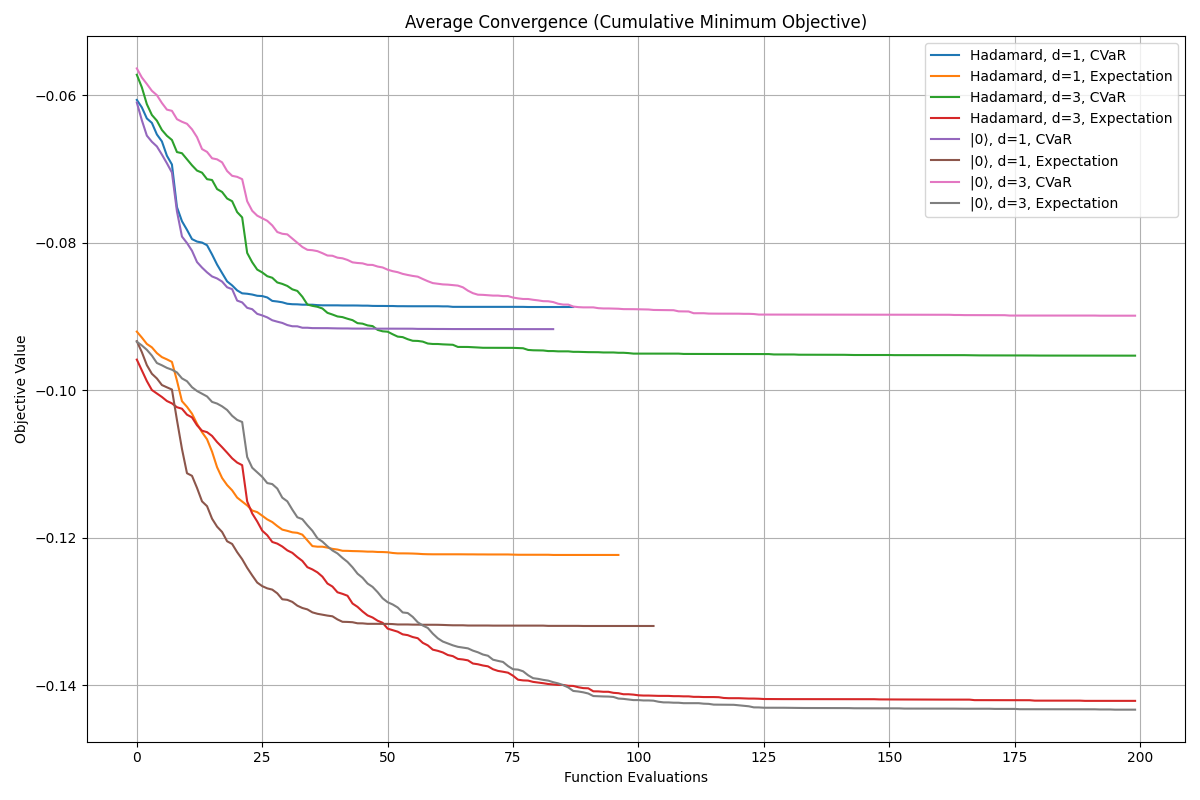
\includegraphics[width=\textwidth]{convergence.png}
\caption{Average convergence profiles showing cumulative minimum objective values
against COBYLA function evaluations. Each line represents the mean trajectory across
20 independent seeds for a given configuration.}
\label{fig:convergence}
\end{figure}

\subsection{Statistical significance}
\label{sec:stats}

Table~\ref{tab:wilcoxon} reports Wilcoxon signed-rank test results for all three comparison families, paired by seed.

\begin{table}[h!]
\caption{Wilcoxon signed-rank test results on best cost, paired by seed ($n = 20$). Nominal significance threshold: $p < 0.05$ (uncorrected).}
\label{tab:wilcoxon}
\centering
\resizebox{\textwidth}{!}{%
\begin{tabular}{llll}
\hline
\textbf{Comparison} & \textbf{$W$} & 
\textbf{$p$-value} & \textbf{Significant} \\
\hline
\multicolumn{4}{l}{\textit{Initialization: $|0\rangle$ vs.\ $H$}} \\
\quad $d=1$, Exp  & $67.5$ & $0.4330$ & No \\
\quad $d=1$, CVaR & $67.0$ & $0.4204$ & No \\
\quad $d=3$, Exp  & $22.0$ & $0.9489$ & No \\
\quad $d=3$, CVaR & $33.0$ & $0.1233$ & No \\
\hline
\multicolumn{4}{l}{\textit{Depth: $d=1$ vs.\ $d=3$}} \\
\quad $H$, Exp           & $3.0$ & $0.0008$ & \textbf{Yes} \\
\quad $H$, CVaR          & $8.0$ & $0.0011$ & \textbf{Yes} \\
\quad $|0\rangle$, Exp   & $12.0$ & $0.0013$ & \textbf{Yes} \\
\quad $|0\rangle$, CVaR  & $23.0$ & $0.0064$ & \textbf{Yes} \\
\hline
\multicolumn{4}{l}{\textit{Objective: Exp vs.\ CVaR}} \\
\quad $H$, $d=1$         & $19.0$ & $0.0355$ & \textbf{Yes} \\
\quad $H$, $d=3$         & $0.0$ & $0.0431$ & \textbf{Yes} \\
\quad $|0\rangle$, $d=1$ & $34.0$ & $0.6949$ & No \\
\quad $|0\rangle$, $d=3$ & $0.0$ & $0.0014$ & \textbf{Yes} \\
\hline
\end{tabular}%
}
\end{table}

Three points follow. First, no initialization comparison reaches significance ($p \geq 0.123$); differences between Hadamard and $|0\rangle$ remain directionally consistent but statistically indistinguishable at $n = 20$, and the study may be underpowered to detect small effects. Second, all four depth comparisons are significant ($p \leq 0.0064$), consistent with deeper circuits providing greater capacity. Third, objective comparisons are nominally significant in three of four cases ($p \leq 0.0431$); however, these $p$-values are uncorrected for multiple comparisons, and the borderline cases ($p = 0.0355$, $p = 0.0431$) may not survive correction.

\subsection{Extended Experiments on a 12-Asset Universe}
\label{sec:extended}

To validate the findings on a larger problem instance, we extend the experiments to $n = 12$ NASDAQ-listed assets (AAPL, MSFT, GOOG, AMZN, META, NVDA, TSLA, JPM, JNJ, V, PG, UNH) with circuit depths $d \in \{1, 2, 3, 4\}$, yielding $4 \times 2 \times 2 \times 20 = 320$ optimization runs. Both $n = 7$ and $n = 12$ remain classically tractable by exhaustive enumeration; these experiments therefore probe optimizer behaviour rather than quantum computational advantage. The classical optimum is obtained by evaluating all $2^{12} - 1 = 4095$ non-empty portfolios, giving $\mathcal{C}^* = -0.1642$. All other experimental parameters (optimizer, shots, seeds) are identical to the 7-asset setting.

Table~\ref{tab:s95_t95} reports the convergence metrics $S_{95}$ and $T_{95}$ for all 16 configurations.

\begin{table}[t]
\caption{Convergence metrics for the 12-asset experiments. $S_{95}$: fraction of 20 seeds reaching $r \geq 0.95$. $T_{95}$: mean iterations to first reach $r_k \geq 0.95$ (computed over all 20 seeds, with non-converging runs capped at 200).}
\label{tab:s95_t95}
\centering
\begin{tabular}{lllcc}
\hline
\textbf{Init} & \textbf{$d$} & \textbf{Obj} & \textbf{$S_{95}$} & \textbf{$T_{95}$} \\
\hline
$H$         & 1 & Exp  & 0.05 & 128.2 \\
$H$         & 1 & CVaR & 0.00 & 132.8 \\
$H$         & 2 & Exp  & 0.60 & 21.0  \\
$H$         & 2 & CVaR & 0.20 & 45.2  \\
$H$         & 3 & Exp  & 0.45 & 28.1  \\
$H$         & 3 & CVaR & 0.20 & 39.6  \\
$H$         & 4 & Exp  & 0.60 & 8.2   \\
$H$         & 4 & CVaR & 0.35 & 8.4   \\
\hline
$|0\rangle$ & 1 & Exp  & 0.10 & 86.2  \\
$|0\rangle$ & 1 & CVaR & 0.05 & 124.2 \\
$|0\rangle$ & 2 & Exp  & 0.50 & 37.5  \\
$|0\rangle$ & 2 & CVaR & 0.10 & 64.5  \\
$|0\rangle$ & 3 & Exp  & 0.45 & 20.6  \\
$|0\rangle$ & 3 & CVaR & 0.25 & 41.0  \\
$|0\rangle$ & 4 & Exp  & 0.45 & 7.1   \\
$|0\rangle$ & 4 & CVaR & 0.40 & 5.5   \\
\hline
\end{tabular}
\end{table}

\subsection{Convergence Analysis}

Among the factors varied in this study, circuit depth has the largest effect on convergence speed. At $d = 1$, virtually no configuration reaches 95\% optimality within 200 iterations: $S_{95} \leq 0.10$ across all initializations and objectives, with $T_{95}$ exceeding 86 iterations on average (note that at such low $S_{95}$, $T_{95}$ is dominated by the 200-iteration ceiling and should not be interpreted as a genuine convergence time). Going from $d = 1$ to $d = 2$ produces the largest improvement, with $S_{95}$ rising from 0.05--0.10 to 0.50--0.60 under Expectation. Further increases to $d = 3$ and $d = 4$ yield modest gains in success rate but large gains in convergence speed: $T_{95}$ drops from 21--37 iterations at $d = 2$ to 5--8 iterations at $d = 4$.

\subsection{Effect of Circuit Depth on Convergence}
Depth brings diminishing returns in success rate but accelerating returns in convergence speed. The largest jump occurs between $d = 1$ and $d = 2$: the parameter count doubles from 12 to 24 and a second entanglement round is added, increasing the expressibility of the variational circuit. Beyond $d = 2$, additional depth mainly speeds up convergence rather than raising the fraction of seeds that reach the target. $S_{95}$ does not increase monotonically with depth in all configurations: for Hadamard-Expectation, it drops from 0.60 at $d = 2$ to 0.45 at $d = 3$ before recovering to 0.60 at $d = 4$; a similar pattern appears for $|0\rangle$-Expectation (0.50 $\to$ 0.45 $\to$ 0.45). With only 20 seeds per configuration, such fluctuations fall within the range expected from sampling variability and should not be over-interpreted. At $d = 4$, runs that reach 95\% optimality do so within 5--8 iterations on average among the converging seeds ($S_{95} = 0.35$--$0.60$).

\subsection{Expectation versus CVaR}
Across the 12-asset experiments, Expectation achieves higher success rates and lower $T_{95}$ than CVaR at every depth. At $d = 2$ with Hadamard initialization, $S_{95}^{\text{Exp}} = 0.60$ versus $S_{95}^{\text{CVaR}} = 0.20$; at $d = 4$, $S_{95}^{\text{Exp}} = 0.60$ versus $S_{95}^{\text{CVaR}} = 0.35$. The Wilcoxon results from the 12-asset runs show significant differences between Expectation and CVaR at $d = 1$ ($p = 0.0006$--$0.0049$) and $d = 2$ ($p = 0.0005$--$0.0012$), with significance diminishing at greater depths ($d = 3$: $p = 0.068$--$0.133$; $d = 4$: $p = 0.021$--$0.127$).
CVaR's lower convergence rate is consistent with its tail-focused evaluation: restricting the objective to the worst $\alpha = 0.3$ fraction of sampled outcomes discards most measurement samples, which produces a noisier signal, complicates COBYLA's local linear model, and leaves fewer successful runs within the 200-iteration budget. CVaR's success rate does rise monotonically with depth, however, as deeper circuits partially compensate for the noisier objective through greater expressibility.
Figures~\ref{fig:boxplot_12}--\ref{fig:s95_depth} present the distribution of approximation ratios, mean convergence trajectories, iterations to 95\% optimality, and success rate as a function of circuit depth for the 12-asset experiments.
\begin{figure}[h!]
\centering
\includegraphics[width=\textwidth]{boxplots.png}
\caption{Distribution of approximation ratios across 20 seeds for the 12-asset experiments. Configurations are grouped by initialization, depth, and objective. The dashed lines mark $r = 1.0$ (global optimum) and $r = 0.95$ (convergence target).}
\label{fig:boxplot_12}
\end{figure}
\begin{figure}[h!]
\centering
\includegraphics[width=\textwidth]{convergence_curves.png}
\caption{Mean convergence trajectories showing cumulative best approximation ratio $r_k$ against function evaluations for the 12-asset experiments. Each curve represents the average across 20 seeds. Horizontal lines mark the global optimum ($r = 1.0$) and convergence target ($r = 0.95$).}
\label{fig:convergence_12}
\end{figure}
\begin{figure}[h!]
\centering
\includegraphics[width=\textwidth]{t95_vs_depth.png}
\caption{Mean iterations to 95\% optimality ($T_{95}$) as a function of circuit depth for the 12-asset experiments, stratified by initialization and objective.}
\label{fig:t95_depth}
\end{figure}
\begin{figure}[h!]
\centering
\includegraphics[width=\textwidth]{success_rate_vs_depth.png}
\caption{Success rate $S_{95}$ (fraction of seeds achieving $r \geq 0.95$) as a function of circuit depth for the 12-asset experiments, stratified by initialization and objective.}
\label{fig:s95_depth}
\end{figure}

\subsection{Discussion}

The interaction between initialization strategy, circuit depth, and objective function is worth examining more closely. At $d = 1$, the circuit has only $n$ trainable parameters and a single entanglement round, limiting its ability to reshape the probability distribution over bitstrings. The slight advantage of Hadamard initialization at shallow depth is likely due to its broader initial coverage of the solution space: Hadamard begins with a uniform probability distribution over all $2^n$ basis states, whereas $|0\rangle$ concentrates all probability mass on a single computational basis state. With relatively few trainable parameters, this broader initial distribution may allow the optimizer to encounter favourable portfolio configurations earlier in the optimization process. The experiments do not directly measure probability-flow dynamics within the circuit, so this interpretation remains a hypothesis.

At $d = 3$, the ansatz has $3n$ parameters and three entanglement rounds, giving it much greater expressibility. The circuit can construct complex probability distributions regardless of the initial state, so the starting point matters less. Under Expectation, $|0\rangle$ and Hadamard perform similarly, consistent with the larger parameter space offering enough pathways to the optimum. Under CVaR, Hadamard retains a small empirical advantage at $d = 3$, though it is not statistically significant. One possible account is that the uniform superposition gives broader early sampling of the portfolio space; since CVaR evaluates only the lowest-cost $\alpha$ fraction of outcomes, early exposure to a more diverse set of bitstrings may improve the quality of the tail distribution seen by the optimizer. This interpretation should be treated cautiously given the lack of significance.

All initialization comparisons remain non-significant under the Wilcoxon test ($p \geq 0.123$ for $n = 7$; $p \geq 0.243$ for $n = 12$). Initialization produces directional shifts early in optimization, but among the factors varied here, circuit depth has the largest effect on solution quality.

The two initialization strategies compared here should not be interpreted as fundamentally different circuit architectures. Within the real-amplitude ansatz considered ($R_Y$ rotations with CNOT entanglement), Hadamard initialization can be viewed as a closely related parameterization of the first variational layer rather than an increase in circuit expressibility. Consequently, any differences observed in this study are more naturally attributed to changes in the optimization trajectory than to differences in representational capacity. This interpretation is consistent with the non-significant Wilcoxon results.
The 12-asset experiments quantify this depth dependence through convergence metrics. $T_{95}$ shows a diminishing-returns pattern: the largest change occurs between $d = 1$ and $d = 2$, where $T_{95}$ drops from $\sim$86--133 to $\sim$21--65 iterations (the $d = 1$ values are ceiling-dominated and do not represent genuine convergence times); further increases to $d = 3$ and $d = 4$ yield progressively smaller gains, with $T_{95}$ reaching $\sim$5--8 iterations at $d = 4$. $S_{95}$ shows a similar threshold effect from $d = 1$ to $d = 2$, jumping from 0.00--0.10 to 0.20--0.60, while the changes from $d = 2$ to $d = 4$ are smaller and not strictly monotonic.

Expectation's advantage over CVaR in the 12-asset setting --- higher $S_{95}$ and lower $T_{95}$ at every depth --- is consistent with CVaR's tail-focused evaluation introducing additional noise that slows convergence within a fixed iteration budget. Restricting the objective to a subset of samples increases estimator variance, which matches this observation.

A few limitations apply. All experiments run on the Qiskit Aer shot-based simulator (\texttt{AerSimulator}) \cite{qiskit}, without gate errors, decoherence, or readout noise; on physical hardware these noise sources could interact with initialization differently. The asset universe is restricted to $n \leq 12$ equities, for which the classical optimum is obtainable by exhaustive enumeration; these experiments therefore characterize optimizer behaviour rather than demonstrating quantum advantage, and scaling to $n = 20$--$30$ assets would test whether the observed trends hold where classical enumeration becomes impractical. Only one ansatz architecture ($R_Y$ rotations with linear CNOT entanglement) and one optimizer (COBYLA) are evaluated; the convergence conclusions may be optimizer-specific, and alternative ans\"atze or optimizers may respond differently to initialization. The fixed COBYLA budget of 200 iterations may penalize deeper circuits with more parameters; adaptive budgets scaled to parameter count should be considered in future work.

Directions for future work include evaluation on noisy quantum backends such as IBM Quantum processors, to determine whether hardware noise amplifies or suppresses the initialization effects seen in simulation; scaling the asset universe beyond the classical tractability threshold; comparison across multiple ansatz families, including QAOA and problem-specific circuits, to clarify whether the initialization--depth--objective interaction is ansatz-dependent; and adaptive initialization schemes where the starting state is chosen based on properties of the cost Hamiltonian.
\section{Conclusion}

We compared qubit initialization strategies --- Hadamard \cite{nielsen2010} versus computational zero-state $|0\rangle$ --- in variational quantum portfolio optimization. Experiments covered 7 and 12 NASDAQ-listed assets under two objective functions (Expectation and CVaR), at circuit depths $d \in \{1, 2, 3, 4\}$, over 20 independent random seeds, yielding 160 runs in the 7-asset setting and 320 in the 12-asset setting.

The main result is that circuit depth has a significant effect on solution quality ($p \leq 0.0064$), while initialization strategy does not reach significance at either problem scale. The study may be underpowered to detect small initialization effects, so the null results should not be taken as evidence that initialization has no effect whatsoever. At $d = 1$, Hadamard initialization produces slightly lower mean cost and variance under both objectives, suggesting more stable optimization when the ansatz has limited expressibility, but these differences are not statistically significant.

The 12-asset experiments confirm these results at a larger scale and extend the analysis through the convergence metrics $T_{95}$ and $S_{95}$. The largest improvement in both success rate and convergence speed occurs between $d = 1$ and $d = 2$; further increases in depth mainly accelerate convergence rather than expand the fraction of successful seeds. Expectation achieves higher success rates ($S_{95}$ up to 0.60 vs.\ 0.35 at $d = 4$). Differences in $T_{95}$ at $d = 4$ are comparatively small (approximately 5--8 iterations across both objectives) and should be interpreted together with the corresponding success rates.

For the ansatz and optimizer tested here, initialization strategy has a smaller effect than circuit depth on variational quantum portfolio optimization. The $d = 1$ to $d = 2$ transition marks the point at which acceptable optimization performance is first achieved in our experiments. All results are from ideal noiseless simulation; the behavior of initialization strategies on physical quantum processors remains open. Future work should include evaluation on noisy hardware, scaling to asset universes where classical enumeration becomes infeasible, testing additional optimizers to determine whether convergence conclusions are optimizer-specific, and comparison across ansatz architectures to test the generality of these observations.

\begin{credits}
\subsubsection{\discintname}
The author has no competing interests to declare that are relevant to the content of this article.
\end{credits}

\begin{thebibliography}{99}
\bibitem{nielsen2010}
M. A. Nielsen and I. L. Chuang, \textit{Quantum Computation 
and Quantum Information}. Cambridge: Cambridge University 
Press, 2010.
\bibitem{cerezo2021}
M. Cerezo et al., ``Variational quantum algorithms,'' 
\textit{Nature Reviews Physics}, vol. 3, no. 9, 
pp. 625--644, 2021.
\bibitem{rockafellar2000}
R. T. Rockafellar and S. Uryasev, ``Optimization of conditional 
value-at-risk,'' \textit{Journal of Risk}, vol. 2, no. 3, 
pp. 21--41, 2000.
\bibitem{markowitz1952}
H. Markowitz, ``Portfolio selection,'' \textit{The Journal 
of Finance}, vol. 7, no. 1, pp. 77--91, 1952.
\bibitem{barkoutsos2020}
P. K. Barkoutsos, G. Nannicini, A. Robert, I. Tavernelli, 
and S. Woerner, ``Improving variational quantum optimization 
using CVaR,'' \textit{Quantum}, vol. 4, p. 256, 2020.
\bibitem{wang2025}
A. Wang, Z. Lv, Z. Ma, D. Cai, and Z. Zhang, ``Achieving
high-quality portfolio optimization with the variational
quantum eigensolver,'' \textit{arXiv preprint arXiv:2508.18625}, 2025.
\bibitem{scursulim2026}
J. V. S. Scursulim, G. M. Langeloh, V. L. Beltran, and
S. Brito, ``Multiclass portfolio optimization via variational
quantum Eigensolver with Dicke state ansatz,''
\textit{Scientific Reports}, vol. 16, no. 1, p. 6208, 2026.
\bibitem{powell1994}
M. J. D. Powell, ``A direct search optimization method 
that models the objective and constraint functions by 
linear interpolation,'' in \textit{Advances in 
Optimization and Numerical Analysis}. Dordrecht: 
Springer, 1994, pp. 51--67.
\bibitem{Farhi2014}
E. Farhi, J. Goldstone, and S. Gutmann, ``A Quantum Approximate Optimization Algorithm,'' \textit{arXiv preprint arXiv:1411.4028}, 2014.
\bibitem{kandala2017hardware}
A. Kandala \textit{et al.}, ``Hardware-efficient variational quantum eigensolver for small molecules and quantum magnets,'' \textit{Nature}, vol. 549, no. 7671, pp. 242--246, 2017.
\bibitem{mcclean2018barren}
J. R. McClean \textit{et al.}, ``Barren plateaus in quantum neural network training landscapes,'' \textit{Nature Communications}, vol. 9, p. 4812, 2018.
\bibitem{Wurtz_2021_fixed_angle}
J. Wurtz and D. Lykov, ``Fixed-angle conjectures for the quantum approximate optimization algorithm on regular MaxCut graphs,'' \textit{Physical Review A}, vol. 104, no. 5, p. 052419, 2021.

\bibitem{qiskit}
A. Javadi-Abhari \textit{et al.}, ``Quantum computing with Qiskit,'' \textit{arXiv preprint arXiv:2405.08810}, 2024.
\bibitem{yfinance}
R. Aroussi, ``yfinance: Download market data from Yahoo! Finance's API,'' GitHub repository, 2026. [Online]. Available: https://github.com/ranaroussi/yfinance
\end{thebibliography}

\end{document}